\section{Methodology} \label{sec:meth}

This section describes our evaluation methodology for evaluating proximate and running the
proximate parallel programs.

\subsection{Workloads}
We first describe the workloads we have targeted and then the methodology to 
evaluate them. Since, proximate is aimed at high performance and throughput
for both regular and irregular workloads, we have considered both class of workloads
and their parallel implementations. 

\paragraph{Regular Workloads}
Regular workloads are generally the high-performance computing applications
which have following properties: i) regular streaming memory access patterns,
ii) Computationally intensive and iii) ample amount of data-level parallelism.
We consider deep learning neural networks kernels similar to Diannao accelerator engine~\cite{diannao}
and the convolution based image processing workloads from Convolution Engine~\cite{convolution_engine}.
Some other micro-benchmarks for functional evaluation considered are: Ocean, summation and reduction, 
but we don't consider in our performance evaluation. 


\paragraph{Irregular Workloads}
Irregular workloads generally have i) irregular memory access patterns
with low ILP, ii) Very small computations and iii) Data dependent control. 
For such workloads, we consider the graph based workloads like histogram, 
shortest path and breadth-first-search. 

\paragraph{}The workloads are further explained in detail here:
The deep neural networks (DianNao~\cite{diannao}) workload suite is regular workloads with 3 benchmarks: Convolution, Pooling, and Classifier. 
Convolution applies local filters to the input data, which is used to find the synaptic weight between feature maps. 
Therefore, convolution is a application with nest matrix multiplication using a sliding window. 
Pooling aggregates data among a set of neighboring input data, which is used for 
extracting and scaling key features. Therefore, pooling is a
tiling matrix reduction workload. 
Classifier aggregates all feature maps and classify the object. Classifier is therefore a matrix-vector multiplication workload. 

The image processing (Conv. engine~\cite{convolution_engine}) workload suite is regular workloads with 3 benchmarks: IME-SAD, SIFT-Blur, and SIFT-DoG. 
Sum of Absolute Difference (SAD) is a 2D kernel to take the difference between 2 images for integer motion estimation (IME). 
IME computes the motion vector by searching for an image block’s closest match to the reference. 
IME can be used in video compression by encoding image blocks and their motions, 
as opposed to encoding every pixel of every frame. Blur is a 1D convolution used for 
blurring images for Scale Invariant Feature Transform (SIFT).
SIFT looks for distinctive features for object detection in images. 
Difference of Gaussian (DoG) is a 2D matrix subtraction operation that can also be used for SIFT. 
The extremas of the DoG pyramid shows the features of interest. 

The irregular workloads explored are breadth first search (bfs), sssp (single source shortest path), and histogram. 
Breadth first search is an algorithm for searching a graph data structure. Bfs starts at the root node and 
explores all neighboring nodes before the next level neighbors, which matches the application of a task queue. 
Sssp finds the minimum cost path from source s to every other vertex. Sssp works on the node with the shortest path, 
and then add all its’ neighbors to the work queue.
Multiple tasks can be executed concurrently with some scheduling to ensure that the task that gives each vertex the
shortest path. Histogram reads every pixel of an image, and sums up the number of pixels with red/green/blue with values 
of 0/1/2/.../254/255. Histogram shows the color (RGB) value (0 through 255) frequency. 
Histogram is an irregular workload because it accesses/increments a color value count. 



\subsection{Simulation Methodology} 
For proximate multi-core riscv inorder core simulation, 
we consider a multi-core simulator called ZSim~\cite{sanchez2013zsim}, which is a
fast x86-65 simulator. It is based on dynamic binary translation and PIN~\cite{pin} model which natively 
runs the pthread instances of the kernel on the real hardware.  

\begin{figure}[h]
  \begin{center}
    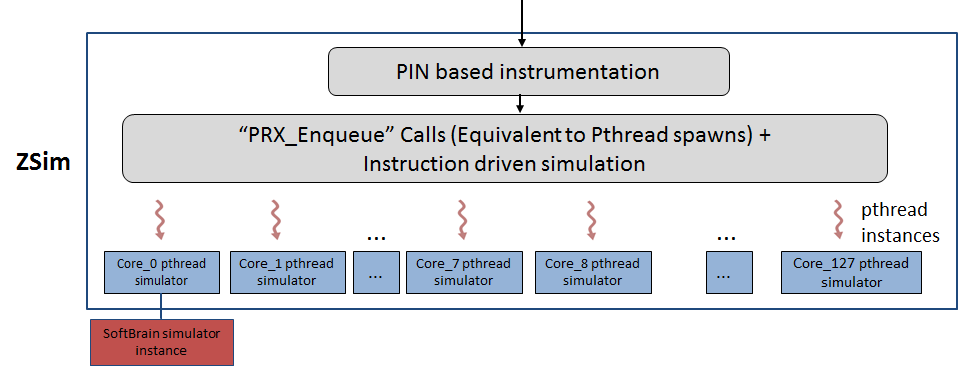
\includegraphics[width=\linewidth]{cs758-figs/zsim-meth.png}
  \end{center}
\vspace{-0.2in}
  \caption{ZSim based Proximate Simulation}
  \label{fig:sim}
\vspace{-0.05in}
\end{figure}

Figure~\ref{fig:sim} shows our simulation methodology, and  each compiled
proximate API based pthread program ins instrumented for multi-core simulation initially.
Then, the proximate API based hooks would identify the proximate kernel and whenever ZSim main thread
encounters a \emph{PRX\_Enqueue} API call, it would offload the kernel to 
a) multiple in-order core pthread instances - if the kernel is an irregular type,  or b) Softbrain simualtor instance
which runs the softbrain portion of the kernel, if the kernel is a regular type. 
Currently, we don't have simulator support to run, multiple instances of Softbrain kernels, 
and hence all the softbrain based parallel kernels need to be serialized to the same softbrain
simulator instance. We aim to support this in our infrastructure in coming days. 

\subsection{Proximate Configurations}
In this section, we explain different configurations of proximate we have simulated, 
to compare against the real hardware. 

\begin{table}[h]
  \centering
  \begin{tabular}{|l|l|}
    \hline
    \textbf{Baseline Configuration} & \textbf{Explanation}                                \\ \hline
    \textit{pthread\_xeon}  & Pthread program run on a 64-core Xeon-Phi processor \\ \hline
    \textit{omp\_xeon}      & OpenMP program run on a 64-core Xeon-Phi processor  \\ \hline
  \end{tabular}
  \caption{Baseline Xeon-Phi configurations used for comparison}
  \label{tab:base-config}
\end{table}

For comparison of parallel program execution on proximate with
a server class processor, we first the baseline versions of parallel programs implemented in pthreads and OpenMP
running on r a 64-core 4way SMT Xeon-Phi processor.
Table~\ref{tab:base-config} explains the 2 baseline versions of parallel programs we run on Xeon-Phi machine.
We vary the number of threads for these 2 baselines, to find out the best design space w.r.t number of threads
and choose that as the comparison point for proximate parallel program.

We now explain, the actual Proximate configurations simulated using the methodology explained above. 
As we know that current proximate hardware has \emph{1 host-core + 128 in-order cores + 1 Softbrain}, we try
to support the same hardware configuration in our simulations. Although, ideally you would be needing 8 Softbrain 
instances running on each vault, our infrastructure cannot support that for now and hence only 1 softbrain.

Based on kernel type, each proximate program can be simulated only on in-order cores without the queueing model
explained previously here in Section~\ref{sec:queue}. Or, if more kernel instances are present in the program, then they 
can be dynamically spawned on the queuing model of proximate. When you have softbrain portions in the program, 
you would want to run on softbrain only simulation. So, there are different ways of simulating proximate based on the kernel
type and Table~\ref{tab:real-configs} summarize the possible simulated configurations for proximate. We would be using these
configurations for comparison in our evaluation. 


\begin{table}[]
  \centering
  \begin{tabular}{|l|l|}
    \hline
    \textbf{Proximate Configuration}               & \textbf{Explanation}                                                    \\ \hline
    \textit{prx\_inorder}                          & Proximate API pthread program w/o queuing model                         \\ \hline
    \textit{prx\_inorder\_q}                       & Proximate API pthread program with queuing model                        \\ \hline
    \textit{prx\_sb\_only}                         & Proximate API + single SoftBrain ‘only’ program                         \\ \hline
    {\color[HTML]{FE0000} \textit{prx\_multi\_sb}} & {\color[HTML]{FE0000} Proximate API + multi-threaded SoftBrain program -- Not simulated} \\ \hline
  \end{tabular}
  \caption{Proximate Simulated Configurations}
\label{tab"real-configs}
\end{table}
